
\FloatBarrier
\section{Map-based Skeletons}
\label{sec:map-skeletons}
Now we have developed Parallel Arrows far enough to define some algorithmic skeletons useful to an application programmer.
\subsection{Parallel map}
\begin{figure}[h]
	\includegraphics[scale=0.7]{images/parMap}
	\caption{Schematic depiction of parMap}
	\label{fig:parMapImg}
\end{figure}
\inlinecode{parMap} (Fig.~\ref{fig:parMapImg},~\ref{fig:parMap}) is probably the most common skeleton for parallel programs. We can implement it with \inlinecode{ArrowParallel} by repeating an arrow \inlinecode{arr a b} and then passing it into \inlinecode{parEvalN} to get an arrow \inlinecode{arr [a] [b]}.
Just like \inlinecode{parEvalN}, \inlinecode{parMap} is 100 \% strict.
\begin{figure}[h]
\begin{lstlisting}[frame=htrbl]
parMap :: (ArrowParallel arr a b conf) =>
	conf -> (arr a b) -> (arr [a] [b])
parMap conf f = parEvalN conf (repeat f)
\end{lstlisting}
\caption{Definition of parMap}
\label{fig:parMap}
\end{figure}

\subsection{Lazy parallel map}
\begin{figure}[h]
	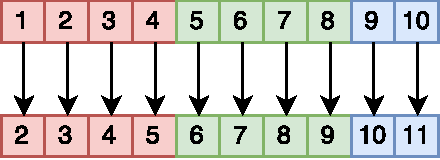
\includegraphics[scale=0.7]{images/parMapStream}
	\caption{Schematic depiction of parMapStream}
	\label{fig:parMapStreamImg}
\end{figure}
As \inlinecode{parMap} (Fig.~\ref{fig:parMapImg},~\ref{fig:parMap}) is 100\% strict it has the same restrictions as \inlinecode{parEvalN} compared to \inlinecode{parEvalNLazy}. So it makes sense to also have a \inlinecode{parMapStream} (Fig.~\ref{fig:parMapStreamImg},~\ref{fig:parMapStream}) which behaves like \inlinecode{parMap}, but uses \inlinecode{parEvalNLazy} instead of \inlinecode{parEvalN}.
\begin{figure}[h]
\begin{lstlisting}[frame=htrbl]
parMapStream :: (ArrowParallel arr a b conf, ArrowChoice arr, ArrowApply arr) =>
	conf -> ChunkSize -> arr a b -> arr [a] [b]
parMapStream conf chunkSize f = parEvalNLazy conf chunkSize (repeat f)
\end{lstlisting}
\caption{Definition of parMapStream}
\label{fig:parMapStream}
\end{figure}

\subsection{Statically load-balancing parallel map}
\begin{figure}[h]
	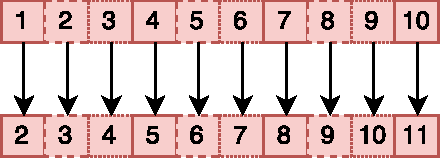
\includegraphics[scale=0.7]{images/farm}
	\caption{Schematic depiction of farm}
	\label{fig:farmImg}
\end{figure}
A \inlinecode{parMap} (Fig.~\ref{fig:parMapImg},~\ref{fig:parMap}) spawns every single computation in a new thread (at least for the instances of \inlinecode{ArrowParallel} we gave in this paper). This can be quite wasteful and a \inlinecode{farm} (Fig.~\ref{fig:farmImg},~\ref{fig:farm}) that equally distributes the workload over \inlinecode{numCores} workers (if numCores is greater than the actual processor count, the fastest processor(s) to finish will get more tasks) seems useful.
\begin{figure}[h]
\begin{lstlisting}[frame=htrbl]
farm :: (ArrowParallel arr a b conf,
	ArrowParallel arr [a] [b] conf, ArrowChoice arr) =>
	conf -> NumCores -> arr a b -> arr [a] [b]
farm conf numCores f =
	unshuffle numCores >>>
	parEvalN conf (repeat (mapArr f)) >>>
	shuffle

unshuffle :: (Arrow arr) => Int -> arr [a] [[a]]
unshuffle n = arr (\xs -> [takeEach n (drop i xs) @|@ i <- [0..n-1]])

takeEach :: Int -> [a] -> [a]
takeEach n [] = []
takeEach n (x:xs) = x : takeEach n (drop (n-1) xs)

shuffle :: (Arrow arr) => arr [[a]] [a]
shuffle = arr (concat . transpose)
\end{lstlisting}
\caption{Definition of farm. \inlinecode{unshuffle}, \inlinecode{takeEach}, \inlinecode{shuffle} were taken from Eden's source code \cite{eden_skel_shuffle}}
\label{fig:farm}
\end{figure}

\subsection{farmChunk}
\begin{figure}[h]
	\includegraphics[scale=0.7]{images/farmChunk}
\caption{Schematic depiction of farmChunk}
\label{fig:farmChunkImg}
\end{figure}
Since a \inlinecode{farm} (Fig.~\ref{fig:farmImg},~\ref{fig:farm}) is basically just \inlinecode{parMap} with a different work distribution, it is, again, 100\% strict. So we define \inlinecode{farmChunk} (Fig.~\ref{fig:farmChunkImg},~\ref{fig:farmChunk}) which uses \inlinecode{parEvalNLazy} instead of \inlinecode{parEvalN}.
\begin{figure}[h]
\begin{lstlisting}[frame=htrbl]
farmChunk :: (ArrowParallel arr a b conf, ArrowParallel arr [a] [b] conf,
	ArrowChoice arr, ArrowApply arr) =>
	conf -> ChunkSize -> NumCores -> arr a b -> arr [a] [b]
farmChunk conf chunkSize numCores f =
	unshuffle numCores >>>
	parEvalNLazy conf chunkSize (repeat (mapArr f)) >>>
	shuffle
\end{lstlisting}
\caption{Definition of farmChunk}
\label{fig:farmChunk}
\end{figure}

\subsection{parMapReduce}
\olcomment{it appears STRANGE. are the data really left alone and noded after map and taken from there by reduce? It makes sense only is no communication through master takes place. ELSE: CUT!}


\mbcomment{this requires some work. Either change this to use futures or cut, yes.}
-- this does not completely adhere to Google's definition of Map Reduce as it
-- the mapping function does not allow for "reordering" of the output
-- The original Google version can be found at https://de.wikipedia.org/wiki/MapReduce

\begin{figure}[h]
\begin{lstlisting}[frame=htrbl]
parMapReduceDirect :: (ArrowParallel arr [a] b conf,
	ArrowApply arr, ArrowChoice arr) =>
	conf -> ChunkSize -> arr a b -> arr (b, b) b -> b -> arr [a] b
parMapReduceDirect conf chunkSize mapfn foldfn neutral =
	arr (chunksOf chunkSize) >>>
	parMap conf (mapArr mapfn >>> foldlArr foldfn neutral) >>>
	foldlArr foldfn neutral
\end{lstlisting}
\caption{Definition of parMapReduceDirect}
\label{fig:parMapReduceDirect}
\end{figure}


%%% Local Variables:
%%% mode: latex
%%% TeX-master: "main"
%%% End:
